\icode{E-MD-CA-L2-261111-001}
如图所示，质量 \(M =\) \,\qty{4}{kg}、长 \(L =\) \,\qty{3}{m}的薄木板静置在水平地面上，质量 \(m =\) \,\qty{1}{kg}的小滑块（可视为质点）以速度 \(v_0 =\) \,\qty{4}{m/s}从木板的左端水平冲上木板，已知滑块与木板间的动摩擦因数 \(\mu = 0.4\)，\(g\) 取\qty{10}{m/s^2}。
\begin{enumerate}
	\item 若木板固定，求滑块相对于木板滑行的最大距离；
	\item 若木板不固定，且水平地面光滑，求滑块相对木板滑行的最大距离。
\end{enumerate}

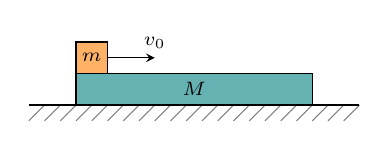
\begin{tikzpicture}[>=stealth,font=\scriptsize]
	\draw[fill=orange!60] (0,.4) rectangle(.4,.8)node[midway]{\(m\)};
	\draw[fill=teal!60] (0,0) rectangle(3,.4)node[midway]{\(M\)};
	\draw[->] (.4,.6)--++(.6,0)node[above]{\(v_0\)};
	\foreach \x in {-.6,-.4,...,3.6}
		\draw[gray] (\x,-.2)--++(.2,.2);
	\draw[thick] (-.6,0)--(3.6,0);
\end{tikzpicture}
\begin{answer}
	（1）\qty{2}{m}（2）\qty{1.6}{m}
\end{answer}